\begin{sloppypar}
In the previous chapters, I showed that despite being relatively new, NMT has already
achieved state-of-the-art translation results for several language pairs 
such as English-French \cite{luong15}, English-German
\cite{jean15,luong15attn,luong15iwslt}, and English-Czech \cite{jean15wmt}. 
While NMT offers many advantages over traditional phrase-based approaches, such as
small memory footprint and simple decoder implementation, nearly all previous
work in NMT has used quite restricted vocabularies, crudely treating all other
words the same with an \unk{} symbol. Sometimes, a post-processing step that
patches in unknown words is introduced to alleviate this problem. %For example,
In Chapter~\ref{c:copy}, I propose to annotate occurrences of target \unk{} with positional information to
track their alignments, after which simple word dictionary
lookup or identity copy can be performed to replace \unk{} in the translation.
\newcite{jean15} approach the problem similarly but obtain the alignments for unknown
words from the attention mechanism. I refer to these as the {\it
unk replacement} technique.
\end{sloppypar}

\begin{figure}%[tbh]
\centering
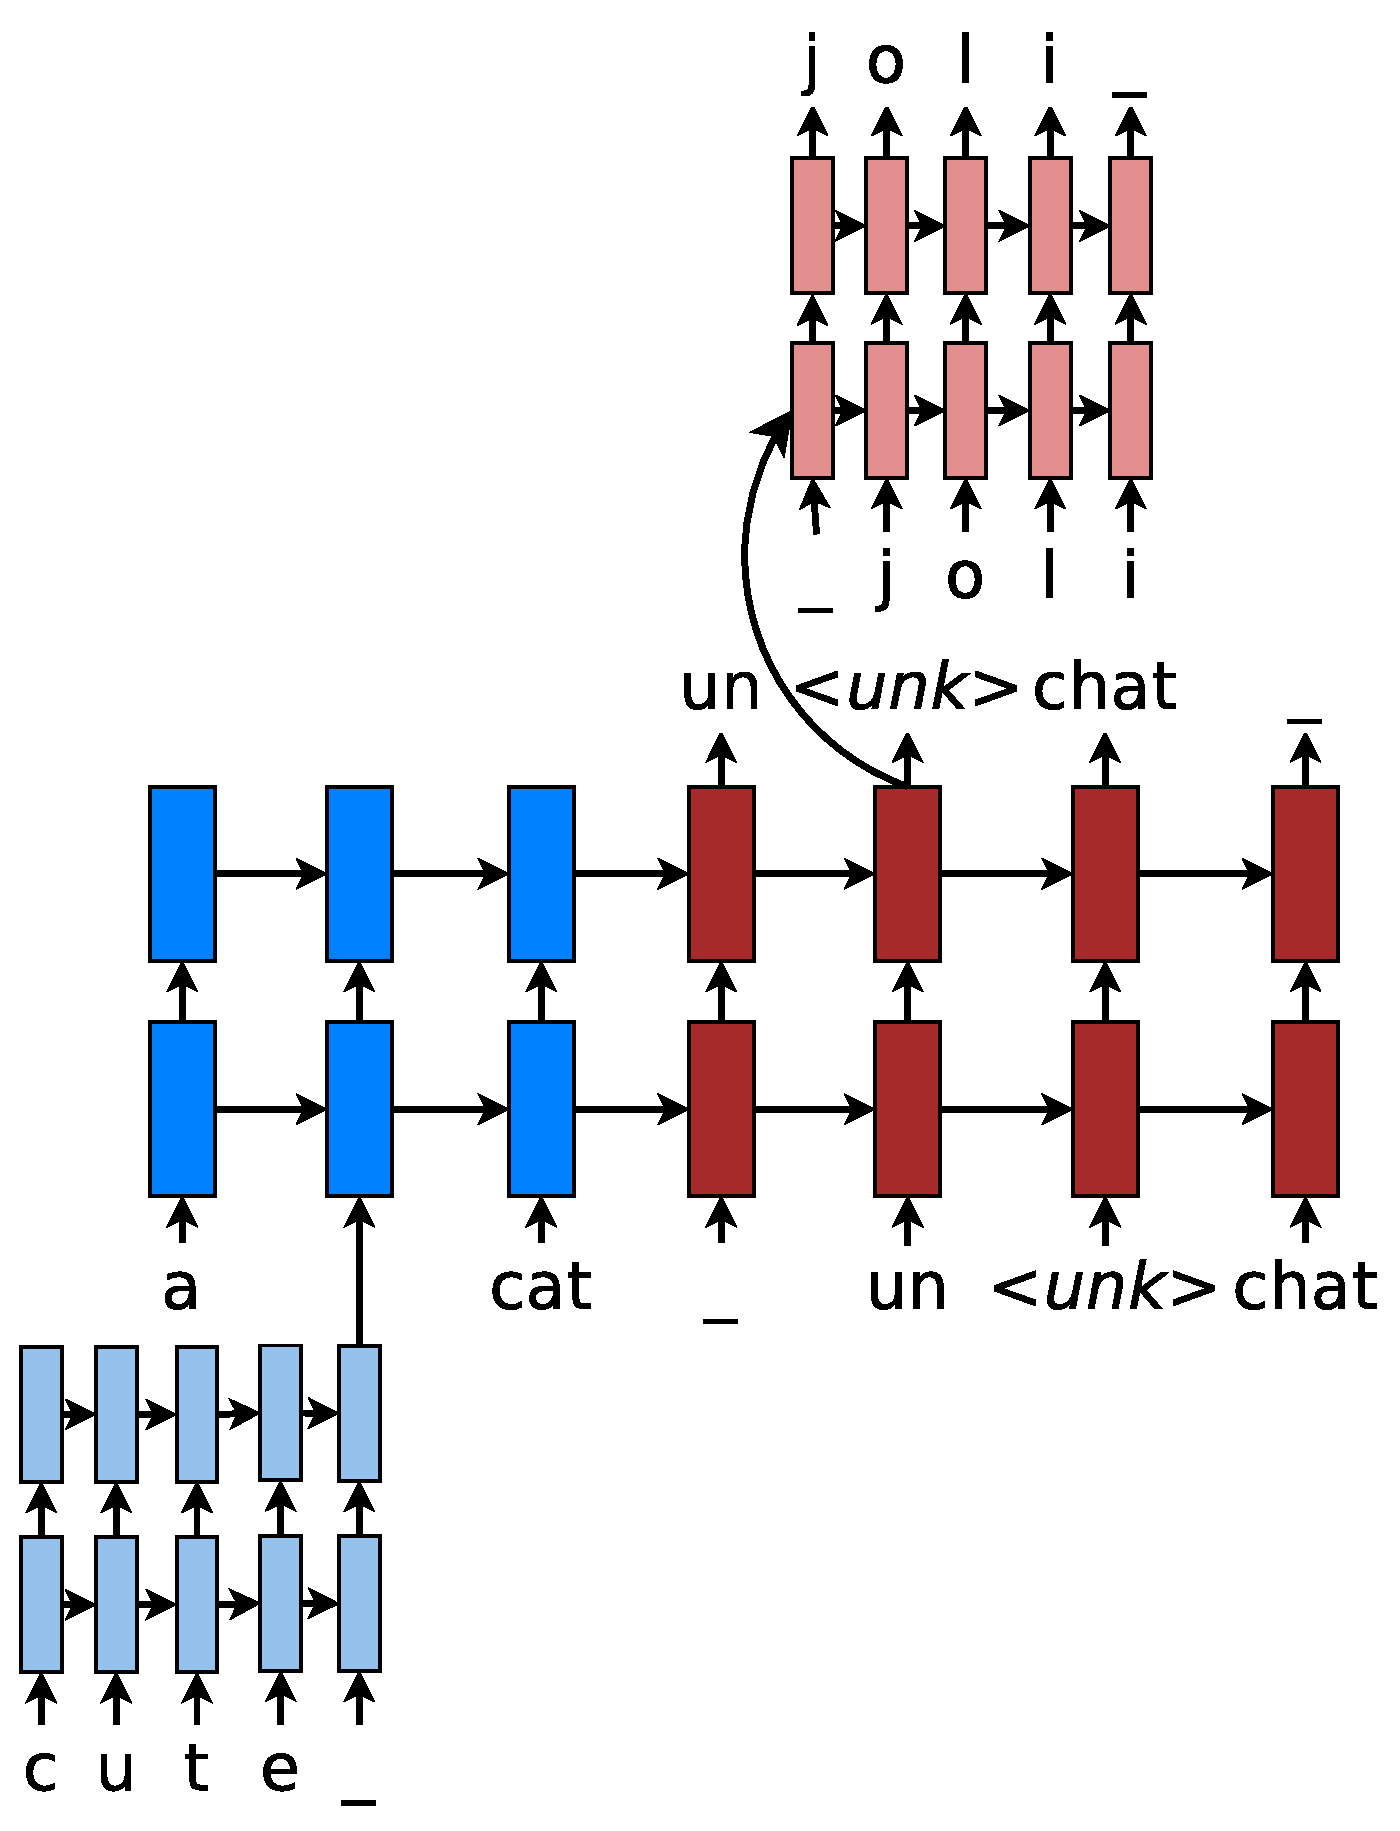
\includegraphics[width=0.6\textwidth, clip=true, trim= 0 0 0 0]{img/5-nmt_hybrid}
\caption[Hybrid NMT]{{\bf Hybrid NMT} -- example of a word-character model for translating
\word{a cute cat} into \word{un
joli chat}. Hybrid NMT translates at the word level. For rare tokens,
the character-level components build source representations
and recover target \unk{}. \word{\_} marks sequence
boundaries.}
\label{f:hybrid}
\end{figure}


Though simple, these approaches ignore several important
properties of languages. First, {\it monolingually}, words are morphologically
related; however, they are currently treated as independent entities. This is
problematic as pointed out by
\newcite{luong13}: neural networks can learn good
representations for frequent words such as \word{distinct}, but fail for
rare-but-related words like \word{distinctiveness}. Second, {\it crosslingually},
languages have different alphabets, so one cannot na\"{i}vely memorize all
possible surface word translations such as name transliteration between 
\word{Christopher} (English) and \word{Kry\u{s}tof} (Czech). See more on this problem
in \cite{sennrich16sub}.

To overcome these shortcomings, I propose a novel {\it hybrid} architecture for NMT
that translates mostly at the word level and consults the character
components for rare words when necessary. As illustrated in
Figure~\ref{f:hybrid}, my hybrid model consists of a word-based NMT that
performs most of the translation job, except for the two (hypothetically) rare words,
\word{cute} and \word{joli}, that are handled separately. On the {\it source}
side, representations for rare words, \word{cute}, are
computed on-the-fly using a deep recurrent neural network that operates at the
character level. On the {\it target} side, I have a separate model that
recovers the surface forms, \word{joli}, of \unk{} tokens character-by-character.
These components are learned jointly end-to-end, removing the need for a separate
unk replacement step as in current NMT practice.

My hybrid NMT offers a twofold advantage: it is much faster and easier to
train than character-based models; at the same time, it never produces unknown
words as in the case of word-based ones.
I demonstrate at scale that on the WMT'15 English to
Czech translation task, such a hybrid approach provides
an additional boost of +$\gain{}$ BLEU points over models 
that already handle unknown words.
I achieve a new state-of-the-art result with
$\ensbleu{}$ BLEU score.
My analysis demonstrates that my character models can successfully learn to not
only generate well-formed words for Czech, a
highly-inflected language with a very complex vocabulary, but also build correct
representations for English source words.

\section{Related Work}
There has been a recent line of work on end-to-end character-based neural models
which achieve good results for part-of-speech tagging \cite{santos14,ling15function},
dependency parsing \cite{ballesteros15}, text classification
\cite{zhang15}, speech recognition \cite{chan16,bahdanau16}, and language
modeling \cite{kim16,rafal16}. However, at the time of this work, success has not been shown for
cross-lingual tasks such as machine translation.
%\footnote{Recently,
%\newcite{ling15char} attempt character-level NMT; however,
%the experimental evidence is weak. The authors demonstrate only small
%improvements over word-level baselines and acknowledge that there are no differences of
%significance. Furthermore, only small datasets were used without
%comparable results from past NMT work.}
\newcite{sennrich16sub} propose to segment words into smaller units and
translate just like at the word level, which does not learn to understand
relationships among words.

My work takes inspiration from \cite{luong13} and 
\cite{li15}. Similar to the former, I build representations for rare words
on-the-fly from subword units. However, instead of using recursive neural
networks with morphemes as units as in \cite{luong13}, which requires existence of a
morphological analyzer, I utilize recurrent neural networks
with characters as the basic units. In comparison with \cite{li15}, my hybrid architecture
is also a hierarchical sequence-to-sequence model, but operates at a different
granularity level, word-character. In contrast, \newcite{li15} build
hierarchical models at the sentence-word level for paragraphs and documents.

\section{Hybrid Neural Machine Translation}
\label{sec:hybrid}
My hybrid architecture, illustrated in Figure~\ref{f:hybrid}, leverages the power of both words
and characters to achieve the goal of open vocabulary NMT. The core of the
design is a {\it word}-level NMT with the advantage of being fast and easy to
train.
The {\it character} components empower the 
word-level system with the abilities to compute any source word representation on the fly from 
characters and to recover character-by-character unknown target words
originally produced as \unk{}.

\subsection{Word-based Translation as a Backbone}
\label{subsec:hybrid_word}
The core of my hybrid NMT is a deep LSTM encoder-decoder that translates at
the {\it word} level as described in Chapter~\ref{c:background}. I maintain a
vocabulary of $|V|$ frequent words for each language. Other words not inside these
lists are represented by a universal symbol \unk{}, one per language.
I translate just like a word-based NMT system with respect to these source and
target vocabularies, except for cases that involve \unk{} in the source input or 
the target output. These correspond to the character-level components 
illustrated in Figure~\ref{f:hybrid}.
A nice property of my hybrid approach is that by varying the vocabulary size,
 one can control how much to blend the
word- and character-based models; hence, taking the best of both
worlds. 


\subsection{Source Character-based Representation}
\label{subsec:src}
In regular word-based
NMT, for all rare words outside the source vocabulary, one feeds the
universal embedding representing \unk{} as input to the encoder. This is
problematic because it discards valuable information about the source word. To
fix that, I learn a deep LSTM model over characters
of source words. 
For example, in Figure~\ref{f:hybrid}, I run
my deep character-based LSTM over `c', `u', `t', `e', and `\_' (the boundary
symbol). The final hidden state at the top layer will be used as the on-the-fly
representation for the current rare word.
The layers of the deep character-based LSTM are always initialized with {\it
zero} states. One might propose to connect hidden
states of the word-based LSTM to the character-based model; however, I chose this design
for various reasons. First, it simplifies the architecture. Second, it allows
for efficiency through {\it precomputation}: before each mini-batch, I can compute
representations for rare source words all at once. All instances of the same
word share the same embedding, so the computation is per {\it type}.\footnote{While \newcite{ling15char} found that it is slow and difficult to train
source character-level models and had to resort to pretraining, I demonstrate
later that I can train my deep character-level LSTM
perfectly fine in an end-to-end fashion.} 

\subsection{Target Character-level Generation}
\label{subsec:tgt}
General word-based NMT allows generation of \unk{} in the target output.
Afterwards, there is usually a post-processing step that handles
these unknown tokens by utilizing the
alignment information derived from the attention mechanism and then performing
simple word dictionary lookup or identity copy \cite{luong15attn,jean15}. 
While this approach works, it suffers from various problems such as alphabet
mismatches between the source and target vocabularies and multi-word
alignments.
My goal is to address all
these issues and create a
coherent framework that handles an unlimited output vocabulary.

My solution is to have a separate deep LSTM that ``translates'' at the
character level given the current word-level state. I train my system such
that whenever the word-level NMT
produces an \unk{}, I can consult this character-level decoder to recover the correct surface form of the
unknown target word. This is illustrated in Figure~\ref{f:hybrid}.
The training objective for the hybrid models consists of two components:
\begin{equation}
J = J_{w} + \alpha J_{c}
\label{e:char_obj}
\end{equation}
Here, $J_{w}$ refers to the usual loss of the word-level NMT; in
my example, it is the sum of the negative log likelihood of
generating $\{\mbox{``un'', ``\unk{}'', ``chat'', ``\_''}\}$. The remaining component $J_c$
corresponds to the loss incurred by the character-level 
decoder when predicting characters, e.g., $\{\mbox{`j', `o', `l', `i',
`\_'}\}$, of those rare words not in the
target vocabulary. 


\paragraph{Hidden-state Initialization}
\label{subsubsec:h}
\begin{figure}
\centering
%\psgrid
\rput(5.6,8.3){$\tgt{t}$}
\rput(1.8,7.2){$\co$}
\rput(1.0,4.1){$\hb{1}$}
\rput(3.7,4.1){$\hb{n}$}
\rput(6.4,4.1){$\hd{t}$}
\rput(6.4,7.8){$\hs$}
%\rput(4.0,3.8){$\hd{t-1}$}
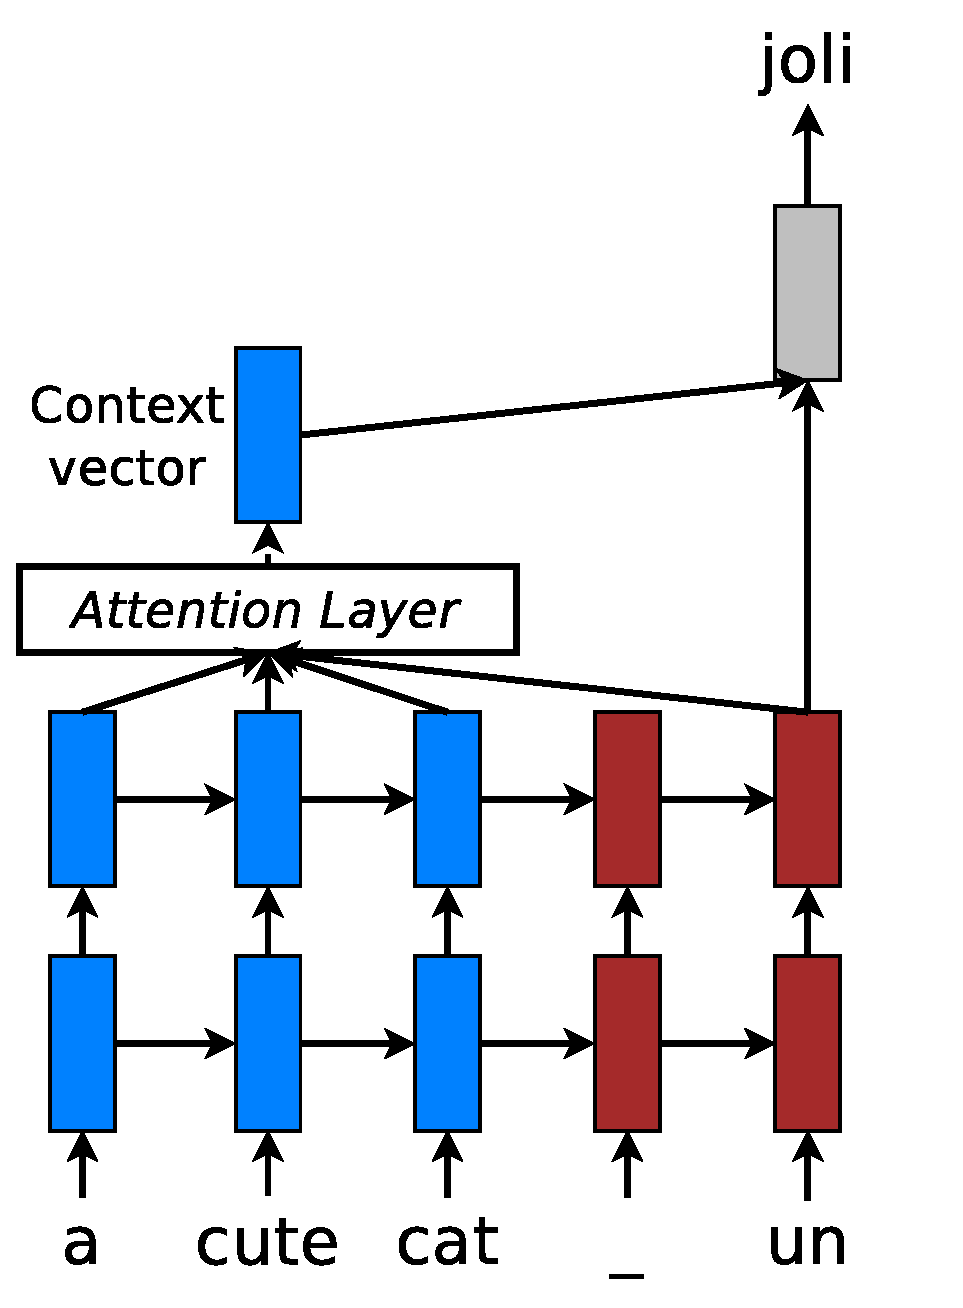
\includegraphics[width=0.45\textwidth, clip=true, trim= 0 0 0 0]{img/5-attn} % , angle=-90
\caption[Attention mechanism]{{\bf Attention mechanism} -- shown are the two steps of the
attention mechanism I described in Chapter~\ref{c:attention} \cite{luong15attn}: first, compute a 
{\it context vector} $\co$ based on the current target hidden state $\hd{t}$ and all the source hidden
states $[\hb{1}, \dots, \hb{n}]$; second, use the context vector as an
additional input to derive
the {\it attentional} vector $\hs$.
} 
\label{f:attn}
\end{figure}

Unlike the source character-based representations, which are
context-independent, the target character-level generation requires the
current word-level context to produce meaningful translation.
This brings up an important
question about what can best represent the current context so as to
initialize the character-level decoder. I answer this question in the context
of the attention mechanism described in Chapter~\ref{c:attention}. 

The final vector $\hs$, just before the
softmax as shown in Figure~\ref{f:attn}, seems to be a good candidate to initialize the character-level decoder.
The reason is that $\hs$ combines
information from both the context vector $\co$ and the top-level recurrent
state $\hi$. I refer to it later in my
experiments as the \textit{same-path} target generation approach.

On the other hand, the same-path approach worries us because all vectors $\hs$
used to seed the character-level decoder might have similar values, leading to
the same character sequence being produced.
The reason is because $\hs$ is directly used in the softmax, \eq{e:softmax}, to predict the same \unk{}.
That might pose some challenges for the model to learn useful representations
that can be used to accomplish two tasks at the same time, that is to predict
\unk{} and to generate character sequences.
To address that concern, I propose another approach called
the \textit{separate-path} target generation.

\begin{figure}%[tbh]
\centering
%\psgrid
\rput(1.8,4.9){$\co$}
\rput(3.2,4.6){$\Wc$}
\rput(5.4,4.6){$\Ww$}
\rput(6.25,1.8){$\hi$}
\rput(3.75,6){$\hc$}
\rput(6.25,6){$\hs$}
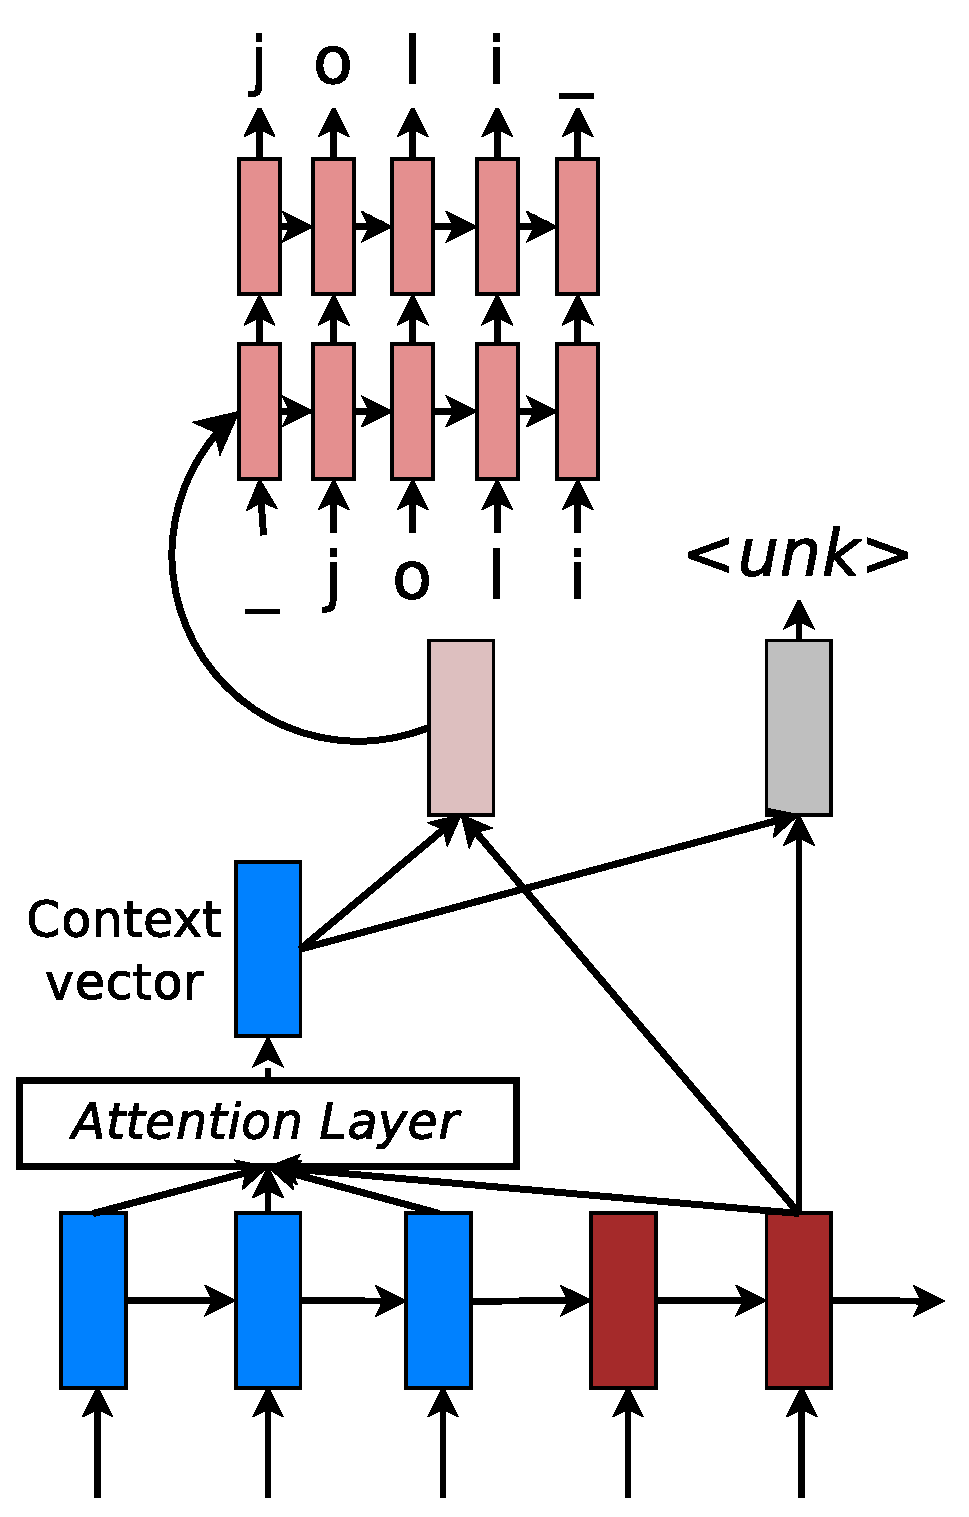
\includegraphics[width=0.45\textwidth, clip=true, trim= 0 0 0 0]{img/5-tgtGen}
\caption[Separate-path target generation]{{\bf Separate-path target generation} -- two separate attentional vectors are creating:
$\hs$ for predicting target words and $\hc$ to seed the target-side character model.}
\label{f:tgtGen}
\end{figure}

My separate-path target generation approach works as follows. I mimic the
process described in \eq{e:hs} of the attention mechanism to create a counterpart vector $\hc$ that will be
used to seed the character-level decoder:
\begin{equation}
\hc = \tanh(\Wc[\co; \hi])
\label{e:hc}
\end{equation} 
Here, $\Wc$ is a new learnable parameter matrix, with which I
hope to release $\W{}$ from the pressure of having to extract information
relevant to both the word- and character-generation processes.
This approach is illustrated in Figure~\ref{f:tgtGen}.
Only the hidden
state of the first layer is initialized as discussed above. The other components
in the character-level decoder such as the
LSTM cells of all layers and the hidden states of higher layers, all start with zero values.

Implementation-wise, the computation in the
character-level decoder is done per word {\it token} instead of per {\it type} as in the source
character component ($\S$\ref{subsec:src}). 
This is because of the context-dependent nature of the decoder.
\footnote{To be memory efficient, the character-level backward pass can be executed right
after the character-level forward pass
and we can split these computations into
mini-batches if the number of \unk{} is large.}

\paragraph{Word-Character Generation Strategy}
\label{subsubsec:strategy}
With the character-level decoder, we can view the final hidden states as representations for
the surface forms of unknown tokens and could have fed these to the next
time step. However, I chose not to do so for the efficiency reason explained
next; instead, \unk{} is fed to the word-level decoder
``as is'' using its corresponding word embedding.

During {\it training}, this design choice decouples all executions over \unk{} instances of the
character-level decoder as soon the word-level NMT
completes. As such, the forward and backward passes of the character-level
decoder over rare words can be invoked in batch mode. At {\it test} time,
my strategy is to first run a beam search decoder at the word level to
find the best translations given by the
word-level NMT. Such translations contains \unk{} tokens, so I utilize the 
character-level decoder with beam search to generate actual words for these \unk{}.

\section{Experiments}
\label{sec:exp}
I evaluate the effectiveness of my models on the publicly available WMT'15
translation task from English into Czech with 
{\it newstest2013} (3000 sentences) as
a development set % to select my hyperparameters. 
and {\it newstest2015} (2656 sentences) as a test set. Two metrics are used: case-sensitive NIST BLEU \cite{Papineni02bleu}
and \chr{} \cite{chrf}.\footnote{For NIST BLEU, I first run
\texttt{detokenizer.pl} % with default setting 
and then use \texttt{mteval-v13a}
to compute the scores as per WMT guideline. For \chr{}, I utilize the implementation here
\url{https://github.com/rsennrich/subword-nmt}.}
The latter measures the amounts of overlapping character $n$-grams and has
been argued to be a better metric for translation tasks out of English.

\subsection{Data}
Among the available language pairs in WMT'15, all involving English, 
I choose {\it Czech} as a target language for several reasons. First and
foremost, Czech is a Slavic language with not only rich
and complex inflection,
but also fusional morphology in which a single morpheme can encode multiple
grammatical, syntactic, or semantic meanings. As a result, Czech possesses an enormously large
vocabulary (about 1.5 to 2 times bigger than that of English according to 
statistics in Table~\ref{t:data}) and is a challenging language to translate
into. Furthermore, this language pair has a large
amount of training data, so %, much bigger than English-Finnish and English-German
I can evaluate at scale. Lastly, though my techniques are language
independent, it is easier for us to work with Czech since Czech uses the Latin alphabet with some
diacritics. % than Russian 

\begin{table} %[tbh!]
\centering
%\resizebox{8cm}{!}{
\begin{tabular}{l|c|c|c|c}
& \multicolumn{2}{c|}{\bf{English}} & \multicolumn{2}{c}{\bf{Czech}}\\
  \cline{2-5}
& word & char & word & char \\
  \hline
  \# Sents & \multicolumn{4}{c}{15.8M} \\
  \hdashline
  \# Tokens & 254M & 1,269M & 224M & 1,347M \\ 
% \hline
% \multicolumn{5}{c}{\biformat{Full}} \\
 \hdashline
  \# Types & 1,172K & 2003 & 1,760K & 2053\\ 
  \hline
  200-char & \multicolumn{2}{c|}{98.1\%} & \multicolumn{2}{c}{98.8\%} \\
\end{tabular}
%}
\caption[WMT'15 English-Czech data]{{\bf WMT'15 English-Czech data} -- shown are various statistics of my training
data such as {\it sentence}, {\it token} (word and character counts), as well as
{\it type} (sizes of the word and character vocabularies).
I show in addition the amount of words in a vocabulary expressed by a list of 200 characters found
in frequent words.}
\label{t:data}
\end{table}

In terms of preprocessing, I apply only the standard tokenization practice.\footnote{I use \texttt{tokenizer.perl} in Moses with
default settings.} I choose for each language a list of 200
characters found in frequent words, which, as shown in Table~\ref{t:data}, can
represent more than 98\% of the vocabulary. 

\begin{table*}%[tbh!]
\centering
\resizebox{15cm}{!}{
\begin{tabular}{c|l|c|c|c|c|c}
 & \multirow{2}{*}{\bf{System}} & \multirow{2}{*}{{\bf
 Vocab}} &
\multicolumn{2}{c|}{{\bf Perplexity}} &\multirow{ 2}{*}{\bf{BLEU}} &\multirow{
2}{*}{\bf{\chr{}}}\\
\cline{4-5}
& & & w & c & & \\
  \hline
(a) & Best WMT'15, big data \cite{bojar15wmt} & % -- {\it large data}
- & - & - & \biformat{18.8} & - \\
  \hline
\multicolumn{7}{c}{{\it Existing} NMT}\\
  \hline
(b) & RNNsearch + unk replace \cite{jean15wmt} & 200K & - & - & 15.7 & - \\
%  \hdashline
(c) & \biformat{Ensemble} 4 models + unk replace \cite{jean15wmt} & 200K & - & - & 18.3 & - \\
  \hline
\multicolumn{7}{c}{My {\it word-based} NMT}\\
  \hline
%(d) & Base & 50K & - & 8.7 & - & 12.6 & 32.8\\
%  \hdashline
(d) & Base + attention + unk replace & 50K & 5.9 & - & 17.5 & 42.4 \\
%  \hdashline
(e) & \biformat{Ensemble} 4 models + unk replace & 50K & - & - & 18.4 & 43.9 \\
  \hline
\multicolumn{7}{c}{My {\it character-based} NMT}\\
  \hline
(f) & Base-512 (600-step backprop) & 200 & - & 2.4 & 3.8 & 25.9\\
(g) & Base-512 + attention (600-step backprop) & 200 & - & 1.6 & 17.5 &
\biformat{46.6} \\
  \hdashline
(h) & Base-1024 + attention (300-step backprop) & 200 & - & 1.9 & 15.7 & 41.1 \\
  \hline
\multicolumn{7}{c}{My {\it hybrid} NMT}\\
  \hline
%(j) & Base + attention + same-path & 1K & 200 & 3.3 & 1.72 & 12.9 (5.0) & 36.3\\
% \hdashline
(i) & Base + attention + same-path & 10K & 4.9 & 1.7 & 14.1 & 37.2 \\
(j) & Base + attention + separate-path & 10K & 4.9 & 1.7 & 15.6 & 39.6 \\
(k) & Base + attention + separate-path + 2-layer char & 10K & 4.7 & 1.6 & \biformat{17.7} & 44.1 \\
% (m) & Base + attention + {\it separate}-path + 2-layer char & 10K & 200 & 4.6 & {\bf 1.59} & \biformat{17.5} (11.3) & 43.4 \\
  \hdashline
(l) & Base + attention + separate-path + 2-layer char & 50K & 5.7 & 1.6 & 19.6 & 46.5 \\
%(n) & Base + attention + {\it separate}-path & 50K & 6.2 & 1.73 & 18.0 (15.5) & 44.4 \\
(m) & \biformat{Ensemble} 4 models & 50K & - & - & {\bf \ensbleu{}} & {\bf 47.5} \\
\end{tabular}
}
\caption[WMT'15 English-Czech results]{{\bf WMT'15 English-Czech results} -- shown are 
the vocabulary sizes, perplexities, BLEU, and \chr{} scores of various systems on
{\it newstest2015}. Perplexities are listed under two
categories, word (w) and character (c). 
% For BLEU scores, I report results before \unk{} tokens are handled in parentheses. 
{\bf Best} and
\biformat{important} results per
metric are highlighted.
% and give {\it progressive} improvements in italic between
% consecutive systems.  
}
\label{t:encs}
\end{table*}


\subsection{Training Details}
I train three types of systems, purely {\it word-based}, purely {\it
character-based}, and {\it hybrid}.
Common to these architectures is a word-based NMT since the
character-based systems are essentially word-based ones with
longer sequences and the core of hybrid models is also a word-based NMT.

In training word-based NMT, I proceed as in Chapter~\ref{c:attention} \cite{luong15attn} to use the global attention mechanism together with
similar hyperparameters: (a) deep LSTM models, 4 layers, 1024
cells, and 1024-dimensional embeddings, (b) uniform initialization of
parameters in $[-0.1, 0.1]$, (c) 6-epoch training with plain SGD and a simple learning
rate schedule -- start with a learning rate of $1.0$; after 4 epochs,
halve the learning rate every 0.5 epoch, (d) mini-batches are of
size 128 and shuffled, (e) the gradient is rescaled whenever its norm exceeds 5, and (f)
dropout is used with probability $0.2$ according to 
\cite{pham2014dropout}.
I now detail differences across the three architectures.

{\bf Word-based NMT} -- I constrain my source and target sequences to
have a maximum length of 50 each; words that go past the boundary are ignored.
The vocabularies are limited to the top $|V|$ most
frequent words in both languages. Words not in these vocabularies
are converted into \unk{}. After translating, I will perform
dictionary\footnote{Obtained from the alignment links produced by the Berkeley
aligner \cite{liang06alignment} over
the training corpus.} lookup or
identity copy for \unk{} using the alignment information from the
attention models. Such a procedure is referred to as the {\it unk replace}
technique as in Chapter~\ref{c:copy} \cite{luong15,jean15}.

{\bf Character-based NMT} -- The source and
target sequences at the character level are often about 5 times longer than their counterparts in the
word-based models as can be inferred from the statistics in
Table~\ref{t:data}. Due to the memory constraint in GPUs, I limit my source and
target sequences to a maximum length of 150 each, i.e., I backpropagate
through at most 300 timesteps from the decoder to the encoder. With
smaller 512-dimensional models, I can afford to have longer sequences with up
to 600-step backpropagation. 

{\bf Hybrid NMT} -- The {\it word}-level component uses the
same settings as the purely word-based NMT. For the {\it character}-level source
and target components, I experiment with both shallow and deep 1024-dimensional models of
1 and 2 LSTM layers. 
I
set the weight $\alpha$ in \eq{e:char_obj} for my character-level loss to
$1.0$.

{\bf Training Time} -- It takes about 3 weeks to train a word-based model with
$|V|=50K$ and about 3 months to train a character-based model. Training and
testing for the hybrid models are about 10-20\% slower than those of the word-based
models with the same vocabulary size.

\subsection{Results}

I compare my models with several strong systems. These include the
winning entry in WMT'15, which was
trained on a much larger amount of data, 52.6M parallel
 and 393.0M monolingual sentences \cite{bojar15wmt}.\footnote{This
entry combines two independent
systems, a phrase-based Moses model and a deep-syntactic transfer-based model.
Additionally, there is  an automatic
post-editing system with hand-crafted rules to correct errors
in morphological agreement and semantic meanings, e.g., loss of negation.}
In contrast, I merely use the
provided parallel corpus of 15.8M sentences.
For NMT, to the best of my knowledge, \cite{jean15wmt} has
the best published performance on English-Czech.

As shown in Table~\ref{t:encs}, for a purely {\it word-based} approach, 
my single NMT model outperforms the best single model in \cite{jean15wmt} by
+$1.8$ points despite
using a smaller vocabulary of only 50K words versus 200K words. 
My ensemble system {\it (e)} slightly outperforms the best previous NMT system with $18.4$ BLEU.

To my surprise, purely {\it character-based} models, though extremely slow to
train and test, perform quite well. The $512$-dimensional attention-based model \modelchar{} is
best, surpassing the single word-based model in
\cite{jean15wmt} despite having much fewer parameters. It even outperforms most NMT
systems  
on \chr{} with $46.6$ points. This indicates that this model translate words that closely but
not exactly match the reference ones as evidenced in
Section~\ref{subsec:samples}. 
I notice two interesting observations. First,
attention is critical for character-based models to work as is obvious from the
poor performance of the non-attentional model; this has also been shown in speech
recognition \cite{chan16}. Second, long time-step backpropagation is more important
as reflected by the fact that the larger $1024$-dimensional model {\it (h)} with shorter
backprogration is inferior to \modelchar{}. 

My {\it hybrid} models achieve the best results. 
At 10K words, I demonstrate that my {\it
separate-path} strategy for the character-level target generation
($\S$\ref{subsubsec:h}) is effective, yielding an improvement of +$1.5$ BLEU
points when comparing systems {\it (j)} vs. {\it (i)}. A {\it deeper} character-level architecture of 2 LSTM
layers provides another significant
boost of +$2.1$ BLEU.
With $17.7$ BLEU points, my hybrid system \modelsmall{} has
surpassed word-level NMT models.

When extending to 50K words, I further improve the translation quality.
My best single model, system \model{} with $19.6$ BLEU, is already better than all
existing systems.
My ensemble model {\it (m)} further advances the SOTA
result to \biformat{\ensbleu} BLEU, outperforming
the winning entry in the WMT'15 English-Czech translation task by a large margin
of +$1.9$ points. My ensemble model is also best in terms of \chr{} with \biformat{47.5} points.

\section{Analysis}
\label{sec:analysis}
This section first studies the effects of vocabulary sizes towards
translation quality. I then analyze more carefully 
my character-level components by visualizing and evaluating rare word
embeddings as well as examining sample translations.

\subsection{Effects of Vocabulary Sizes}
As shown in Figure~\ref{f:vocab}, my hybrid models offer large gains of
+\gain{} BLEU points over strong word-based systems which already handle unknown words.
With only a small vocabulary, e.g., 1000 words, my hybrid approach can produce
systems that are better than word-based models that possess much larger
vocabularies. While it appears from the plot that gains diminish as I
increase the vocabulary size, I argue that my hybrid models are still
preferable since they understand word structures and can handle new complex
words at test time as illustrated in Section~\ref{subsec:samples}.
\begin{figure}
\centering
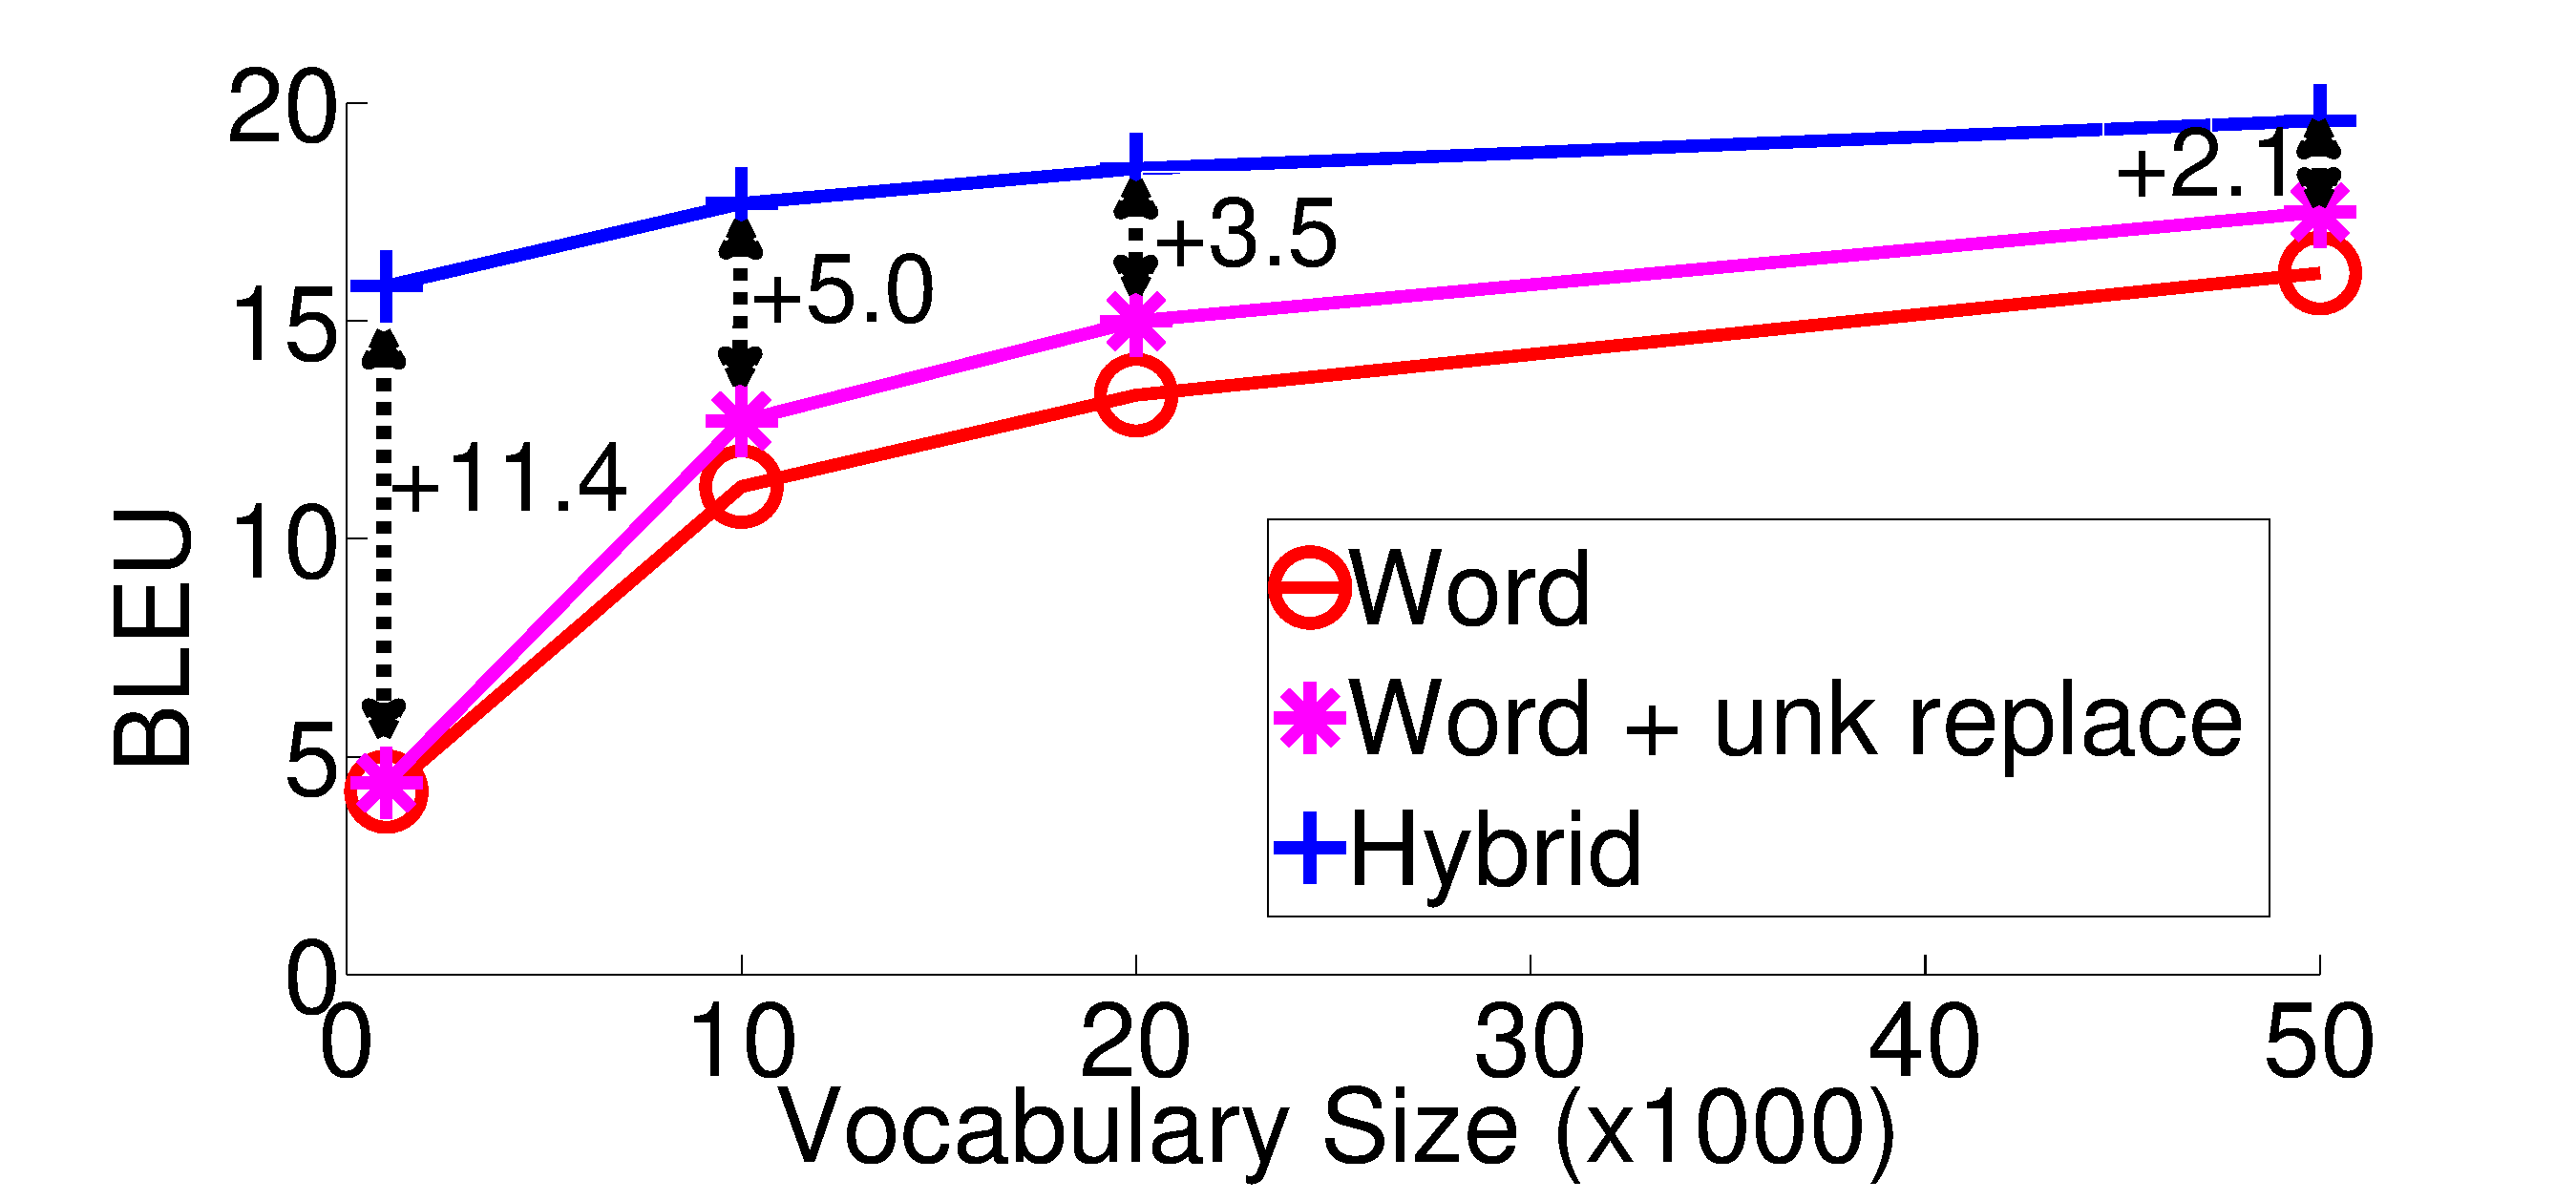
\includegraphics[width=0.7\textwidth, clip=true, trim= 0 0 0 0]{img/5-vocab}
\caption[Vocabulary size effect]{{\bf Vocabulary size effect} -- shown are the performances of different
systems as I vary their vocabulary sizes. I highlight the improvements obtained
by my hybrid models over word-based systems which already handle unknown words.}
\label{f:vocab}
\end{figure}



\subsection{Rare Word Embeddings}
I evaluate the {\it source} character-level model by building representations
for rare words and measuring how good these embeddings are.

Quantitatively, I follow \newcite{luong13} in using the word similarity task,
specifically on the {\it Rare Word} dataset, to judge the learned representations for
complex words. The evaluation metric is the Spearman's correlation $\rho$
between similarity scores assigned by a model and by human annotators.
From the results in Table~\ref{t:word_sim}, I can see that source representations produced by
my hybrid\footnote{I look up the encoder embeddings for frequent words and build representations for
rare word from characters.}  models
are significantly better than those of the word-based one. It is noteworthy that my deep recurrent
character-level models can outperform the model of \cite{luong13}, which uses
recursive neural networks and requires a complex morphological analyzer, by a large
margin. My performance is also competitive to the best Glove embeddings
\cite{pennington2014} which were trained on a much larger dataset.
\begin{table}[tbh!]
\centering
%\resizebox{8cm}{!}{
\begin{tabular}{c|l|c|c|c}
\multicolumn{2}{c|}{{\bf System}} & Size & $|V|$ & \bf{$\rho$}\\ %Spearman's 
  \hline
\multicolumn{2}{l|}{\cite{luong13}} & 1B & 138K & 34.4 \\
  \hdashline
\multicolumn{2}{l|}{\multirow{2}{*}{Glove \cite{pennington2014}}} & 6B & 400K & 38.1 \\
\multicolumn{2}{l|}{} & 42B & 400K & \bf{47.8} \\
  \hline
\multicolumn{4}{c}{{\it My NMT models}}\\
  \hline
\modelword{} & Word-based & 0.3B & 50K & 20.4 \\
  \hdashline
\modelsmall{} & Hybrid & 0.3B & 10K & 42.4 \\
  \hdashline
\model{} & Hybrid & 0.3B & 50K & \biformat{47.1} \\
\end{tabular}
%}
\caption[Word similarity task]{{\bf Word similarity task} -- shown are Spearman's correlation
$\rho$ on the {\it Rare Word} dataset
of various models (with different vocab sizes $|V|$). 
} 
\label{t:word_sim}
\end{table}


Qualitatively, I visualize embeddings produced by the hybrid model \model{} for
selected words in the Rare Word dataset.
Figure~\ref{f:visual} shows the two-dimensional representations of words
computed by the
Barnes-Hut-SNE algorithm \cite{bhsne}.\footnote{I run Barnes-Hut-SNE algorithm
over a set of 91 words, but filter out 27 words for displaying clarity.} It is extremely interesting to observe that
words are clustered together not only by the word structures but also by
the meanings. For example, in the top-left box,
the {\it character}-based representations for \word{loveless}, \word{spiritless}, \word{heartlessly}, and \word{heartlessness} are nearby,
but clearly separated into two groups. Similarly, in the center boxes, {\it
word}-based embeddings of
\word{acceptable}, \word{satisfactory}, \word{unacceptable}, and \word{unsatisfactory}, are
close by but separated by meanings. Lastly, the remaining boxes demonstrate that my
character-level models are able to build representations comparable to the
word-based ones, e.g., \word{impossibilities} vs.\ \word{impossible} and \word{antagonize}
vs.\ \word{antagonist}. All of this evidence strongly supports that the source
character-level models are useful and effective.

\begin{figure*}
\centering
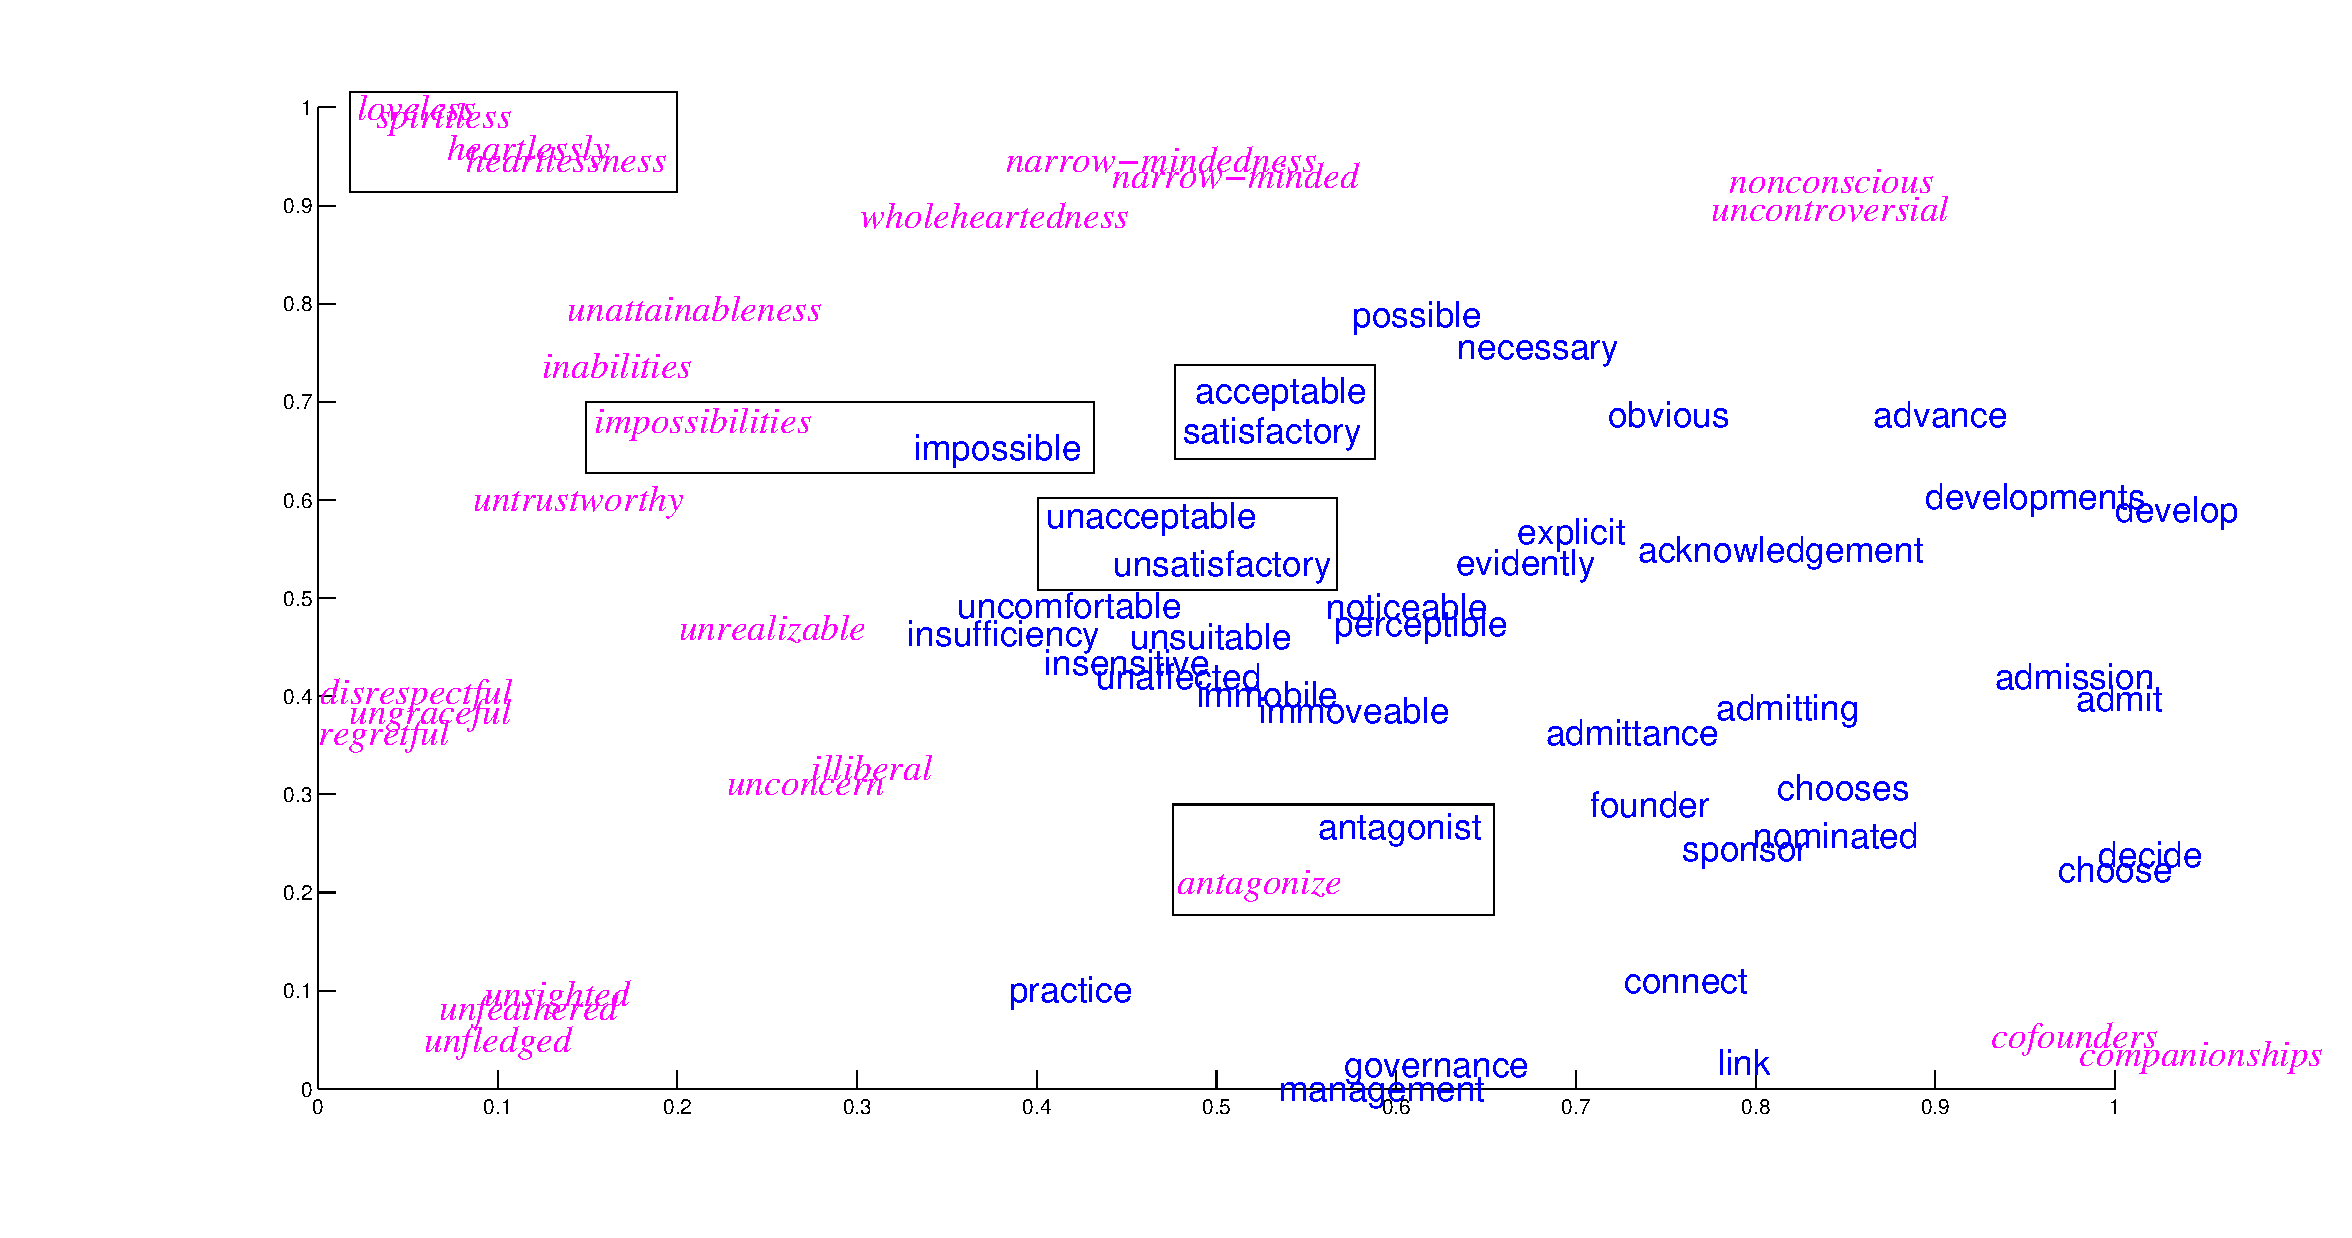
\includegraphics[width=\textwidth, clip=true, trim= 100 50 0 20]{img/5-emb}
\caption[Barnes-Hut-SNE visualization of source word representations]{{\bf Barnes-Hut-SNE visualization of source word representations} --
shown are sample words from the {\it Rare Word} dataset. I differentiate two types of
embeddings: {\color{blue} frequent} words in which encoder embeddings are looked up directly and {\it {\color{magenta} rare}} words
where I build representations from characters. Boxes highlight examples that
I will discuss in the text. I use the hybrid model \model{} in this visualization.}
\label{f:visual}
\end{figure*}


\begin{table*}%[tbh!]
\centering
\resizebox{15cm}{!}{
\begin{tabular}{c|c|p{15.5cm}}
% sent 1046 
\multirow{7}{*}{1} & source & The author \source{Stephen Jay Gould} died 20 years after
\source{diagnosis} . \\
& human & Autor \correct{Stephen Jay Gould} zem\u{r}el 20 let po
\correct{diagn\'oze} . \\
  \cline{2-3}
& \multirow{2}{*}{\it{word}} & Autor Stephen Jay \unk{} zem\u{r}el 20 let po
\unk{} . \\
&  & Autor \correct{Stephen Jay Gould} zem\u{r}el 20 let po \wrong{po} .\\
  \cline{2-3}
& \it{char} & Autor \wrong{Stepher Stepher} zem\u{r}el 20 let po
\correct{diagn\'oze} . \\
  \cline{2-3}
& \multirow{2}{*}{\it{hybrid}} & Autor \unk{} \unk{} \unk{} zem\u{r}el 20 let po
\unk{}. \\
&  & Autor \correct{Stephen Jay Gould} zem\u{r}el 20 let po \correct{diagn\'oze} .\\
  \hline
  \hline
% sent 80
\multirow{7}{*}{2} & source & As the Reverend \source{Martin Luther King
Jr.} said \source{fifty years ago} :\\
& human & Jak \correct{p\u{r}ed pades\'ati lety} \u{r}ekl reverend \correct{Martin
Luther King Jr} . : \\
  \cline{2-3}
& \multirow{2}{*}{\it{word}} & Jak \u{r}ekl reverend Martin \unk{} King \unk{}
p\u{r}ed pades\'ati lety : \\
&  & Jak \u{r}ekl reverend \correct{Martin Luther King} \wrong{\u{r}ekl}
\close{p\u{r}ed pades\'ati lety} : \\
  \cline{2-3}
& \it{char} & Jako reverend \correct{Martin Luther} \wrong{kr\'al \u{r}\'ikal}
\close{p\u{r}ed pades\'ati lety} : \\
  \cline{2-3}
& \multirow{2}{*}{\it{hybrid}} & Jak p\u{r}ed \unk{} lety \u{r}ekl \unk{} Martin
\unk{} \unk{} \unk{} : \\
&  & Jak \correct{p\u{r}ed pades\'ati lety} \u{r}ekl reverend \correct{Martin
Luther King} \close{Jr.} : \\
  \hline
  \hline
% sent 198
\multirow{7}{*}{3} & source & Her \source{11-year-old} daughter , \source{Shani Bart} , said it felt a " little bit
\source{weird} " [..] back to school \\
& human & Jej\'{i} \correct{jeden\'{a}ctilet\'{a}} dcera \correct{Shani Bartov\'{a}} prozradila
, \u{z}e " je to trochu \correct{zvl\'{a}\u{s}tn\'{i}} " [..] znova do
\u{s}koly \\
  \cline{2-3}
& \multirow{2}{*}{\it{word}} & Jej\'i \unk{} dcera \unk{} \unk{} \u{r}ekla , \u{z}e je to " trochu
divn\'e " , [..] vrac\'i do \u{s}koly \\
&  & Jej\'i \wrong{11-year-old} dcera \correct{Shani} \wrong{,} \u{r}ekla , \u{z}e je to " trochu
\close{divn\'e} " , [..] vrac\'i do \u{s}koly \\
  \cline{2-3}
& \it{char} & Jej\'i \correct{jeden\'actilet\'a} dcera , \correct{Shani
Bartov\'a} , \u{r}\'ikala ,
\u{z}e c\'it\'i trochu \close{divn\u{e}} , [..] vr\'atila do \u{s}koly \\
  \cline{2-3}
& \multirow{2}{*}{\it{hybrid}} & Jej\'i \unk{} dcera , \unk{} \unk{} , \u{r}ekla , \u{z}e c\'it\'i " trochu
\unk{} " , [..] vr\'atila do \u{s}koly \\
&  & Jej\'i \correct{jeden\'actilet\'a} dcera , \wrong{Graham} \close{Bart} , \u{r}ekla , \u{z}e c\'it\'i " trochu
\close{divn\'y} " , [..] vr\'atila do \u{s}koly \\
\end{tabular}
}
\caption[Sample translations on newstest2015]{{\bf Sample translations on newstest2015} -- %examples in both translation directions.
for each example, I show the {\it source}, {\it human} translation, and
translations of the following NMT systems: {\it word} model \modelword{},
{\it char} model \modelchar{}, and {\it hybrid} model \modelsmall{}. I show the
translations before replacing \unk{} tokens (if any) for the word-based 
and hybrid models. The following formats are used to highlight
\correct{correct}, \wrong{wrong}, and \close{close} translation segments.}
\label{t:sample}
\end{table*}


\subsection{Sample Translations}
\label{subsec:samples}

I show in Table~\ref{t:sample} sample translations between various systems. 
In the first example, my hybrid model translates perfectly. The word-based
model fails to translate \word{diagnosis} because the second \unk{} was incorrectly
aligned to the word \word{after}. The character-based model, on the other hand,
makes a mistake in translating names.

For the second example, the hybrid model surprises us when it can capture
the long-distance reordering of \word{fifty years ago} and \word{p\u{r}ed
pades\'ati lety} while the other two models do not. The word-based model
translates \word{Jr.} inaccurately due to the incorrect alignment between the
second \unk{} and the word \word{said}. The
character-based model literally translates the name \word{King} into \word{kr\'al}
which means \word{king}.

Lastly, both the character-based and hybrid models impress us by
their ability to translate compound words exactly, e.g., \word{11-year-old} and
\word{jeden\'actilet\'a}; whereas the identity copy
strategy of the word-based model fails.
Of course, my hybrid model does make mistakes, e.g., it fails to translate the name
\word{Shani Bart}. 
Overall, these examples highlight how challenging translating
into Czech is and that being able to translate at the character level helps
improve the quality.

\section{Conclusion}
\label{sec:conclude}
I have proposed a novel {\it hybrid} architecture that combines the strength
of both word- and character-based models. Word-level models are fast to train
and offer high-quality translation; whereas, character-level models help achieve
the goal of open vocabulary NMT. 
I have demonstrated these two aspects through my experimental results and
translation examples.

My best hybrid model has surpassed the performance of both the best word-based
NMT system and the best non-neural model to establish a new state-of-the-art result for 
English-Czech translation in WMT'15 with $\ensbleu{}$ BLEU.
Moreover, I have succeeded in replacing the standard unk replacement technique
in NMT with my character-level components, yielding an improvement of 
+$\gain{}$ BLEU points. My analysis has shown that my model has the ability to
not only generate well-formed words for
Czech, a highly inflected language with an enormous and complex vocabulary, but
also build accurate representations for English source words.
Additionally, I have demonstrated the potential of purely character-based
models in producing good translations;
they have outperformed past word-level NMT models. 
I will further discuss the potential of these models in Chapter~\ref{c:conclude}.
